\part{Using LabPlot}

\chapter{Interface}
\section{Main Area}
\section{Project Explorer}
\section{Properties Explorer}

\chapter{Data Containers}
\section{Spreadsheet}
\section{Matrix}
\section{Workbook}

\chapter{2D Plotting}
\section{Plots}
\section{Curves}
\section{Legends}


% \chapter{3D Plotting}

\chapter{Themes and Templates}


\chapter{Data Analysis}
\section{Data reduction}
\section{Differentiation}
\section{Integration}
\section{Interpolation}
\section{Smoothing}
\section{Curve Fitting}
\section{Fourier Filter}

\newpage
\section{Fourier Fransform}
Available window functions are
\begin{eqnarray*}
\text{rectangular(uniform):} \quad  w(n) &=& 1 \\
\text{triangular:} \quad w(n) &=& 1 - \frac{2}{N} \left| n-\frac{N-1}{2} \right| \\
\text{triangular (Bartlett):} \quad  w(n) &=&  1 - \frac{2}{N-1} \left|n-\frac{N-1}{2}\right| \\
\text{triangular (Parzen):} \quad  w(n) &=& 1 - \frac{2}{N+1} \left| n-\frac{N-1}{2} \right| \\
\text{Welch (parabolic):} \quad  w(n) &=& 1 - \left(2 \frac{n-(N-1)/2}{N+1} \right)^2 \\
\text{Cosine:} \quad  w(n) &=& \sin\left( \frac{\pi n}{N-1} \right) \\
\text{Bartlett-Hann:} \quad  w(n) &=& 0.62 - 0.48 \left| \frac{n}{N-1}-0.5 \right| - 0.38 \cos\left(\frac{2\pi n}{N-1}\right) \\
\text{Lanczos:} \quad  w(n) &=& \mathrm{sinc} \left(\frac{2n}{N-1}-1\right) \\
\end{eqnarray*}

Higher-order generalized cosine window functions:
\begin{eqnarray*}
\text{Hann (raised cosine):} \;  w(n) &=& 0.5 - 0.5 \cos \left(\frac{2 \pi n}{N-1}\right) \\
%
\text{Hamming:} \;  w(n) &=& 0.54 - 0.46 \cos\left( \frac{2\pi n}{N-1} \right) \\
%
\text{Blackman:} \;  w(n) &=& 0.42 - 0.5 \cos\left(\frac{2\pi n}{N-1}\right) + 0.08 \cos\left(\frac{4\pi n}{N-1} \right) \\
%
\text{Nuttall:} \;  w(n) &=& a_0 + a_1 \cos\left(\frac{2\pi n}{N-1}\right) + a_2 \cos\left(\frac{4\pi n}{N-1}\right) + a_3 \cos\left(\frac{6\pi n}{N-1}\right) \\
&& a_0 = 0.355768,\; a_1 =  -0.487396,\; a_2 = 0.144232,\; a_3 = -0.012604 \\
%
\text{Blackman-Nuttall:} \;  w(n) &=& a_0 + a_1 \cos\left(\frac{2\pi n}{N-1}\right) + a_2 \cos\left(\frac{4\pi n}{N-1}\right) + a_3 \cos\left(\frac{6\pi n}{N-1}\right) \\
&& a_0 = 0.3635819,\; a_1 =  -0.4891775,\; a_2 = 0.1365995,\; a_3 = -0.0106411 \\
%
\text{Blackman-Harris:} \;  w(n) &=& a_0 + a_1 \cos\left(\frac{2\pi n}{N-1}\right) + a_2 \cos\left(\frac{4\pi n}{N-1}\right) + a_3 \cos\left(\frac{6\pi n}{N-1}\right) \\
&& a_0 = 0.35875,\; a_1 =  -0.48829,\; a_2 = 0.14128,\; a_3 = -0.01168 \\
%
\text{Flat top:} \;  w(n) &=& a_0 + a_1 \cos\left(\frac{2\pi n}{N-1}\right) + a_2 \cos\left(\frac{4\pi n}{N-1}\right) +a_3 \cos\left(\frac{6\pi n}{N-1}\right) + a_4 \cos\left(\frac{8\pi n}{N-1}\right); \\
&& a_0 = 1, \; a_1 =  -1.93,\; a_2 = 1.29,\; a_3 = -0.388,\; a_4 = 0.028 \\
\end{eqnarray*}


\chapter{CAS Computing}
LabPlot can be used as a frontend to different open-source computer algebra systems (CAS) like Maxima, Octave, R, Scilab and Sage  or programming languages providing similar capabilities like Python and Julia. LabPlot recognizes different CAS variables holding array-like data and allows to select them as the source for curves. So, instead of providing columns of a spreadsheet as the source for x- and y-data, the user provides the names of the corresponding CAS-variables. Currently supported CAS data containers are
\begin{itemize}
\item \textbf{Maxima} lists
\item \textbf{Python} lists, tuples and NumPy arrays
\item \textbf{Julia} vectors and tuples
\end{itemize}

With this, powerfull calculations carried out inside of different CAS environments can be combined with the user-friendly visualisation and editing capabilities of LabPlot. This combination is demonstrated below with the help of two examples:
\begin{figure}
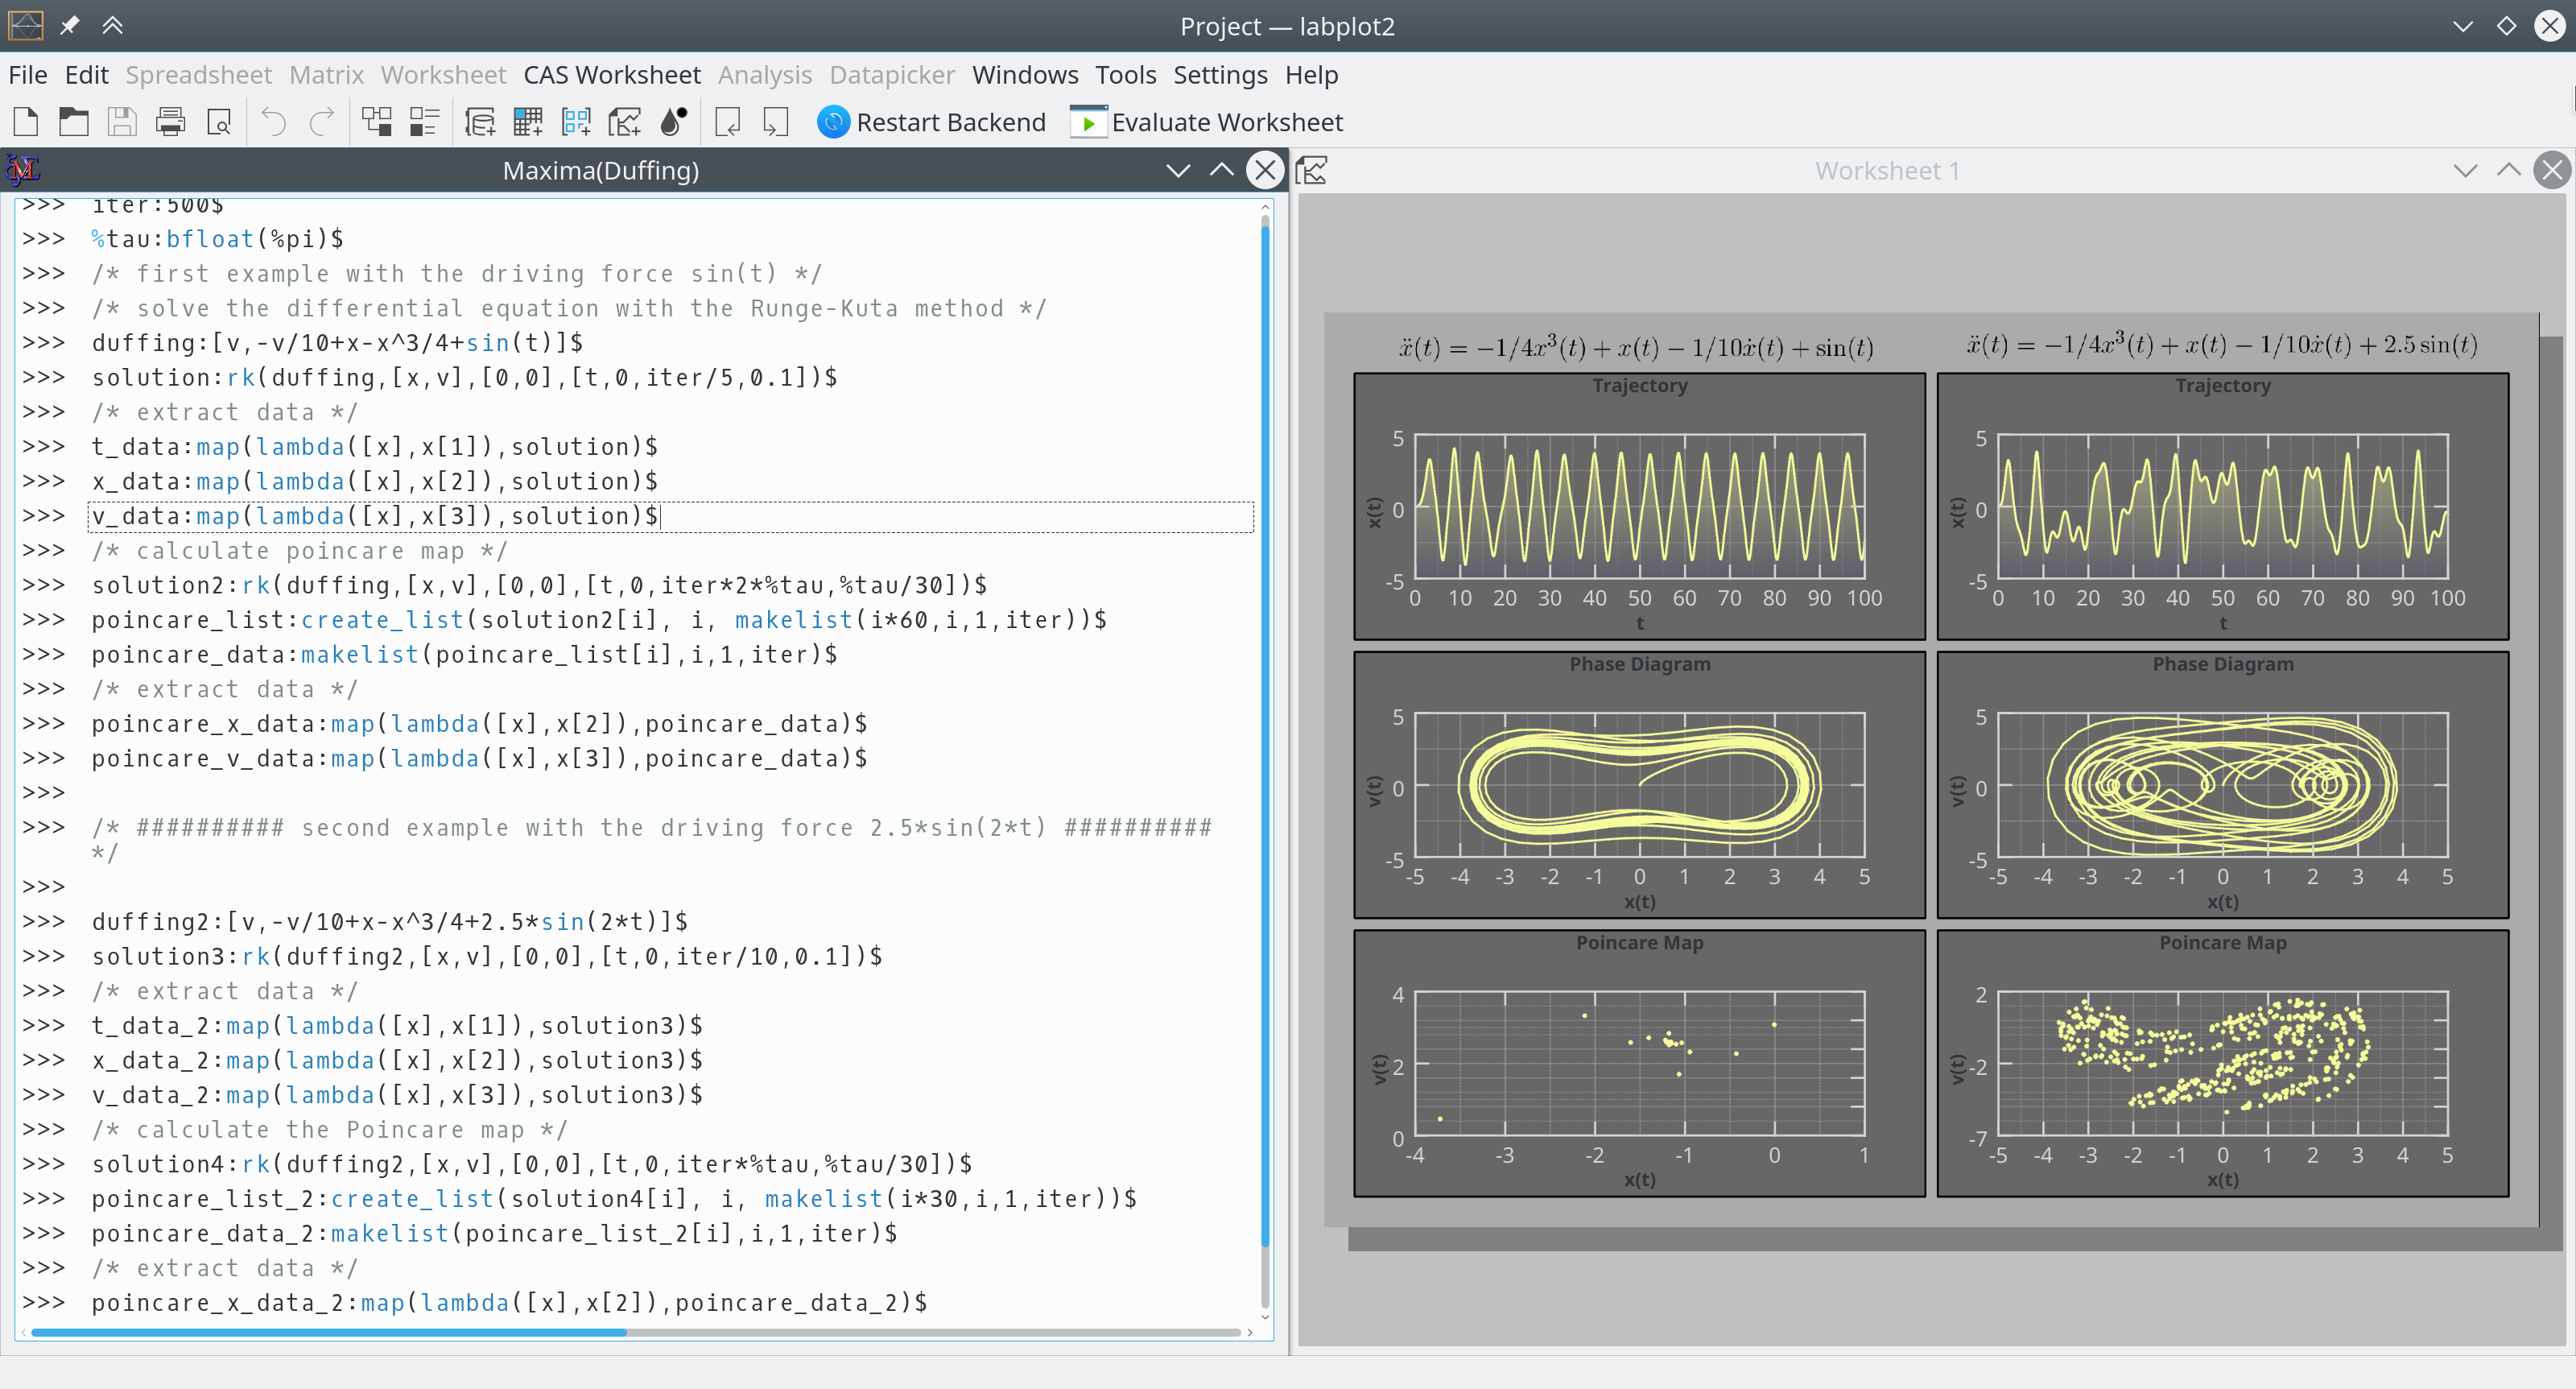
\includegraphics[width=\textwidth]{images/maxima_session.png}
\caption{Maxima session showing the chaotic dynamics of the Duffing oscillator. The differential equation of the forced oscillator is solved with Maxima. Plots of the trajectory, the phase space of the oscillator and the corresponding Poincaré map are done with LabPlot.}
\end{figure}

\begin{figure}
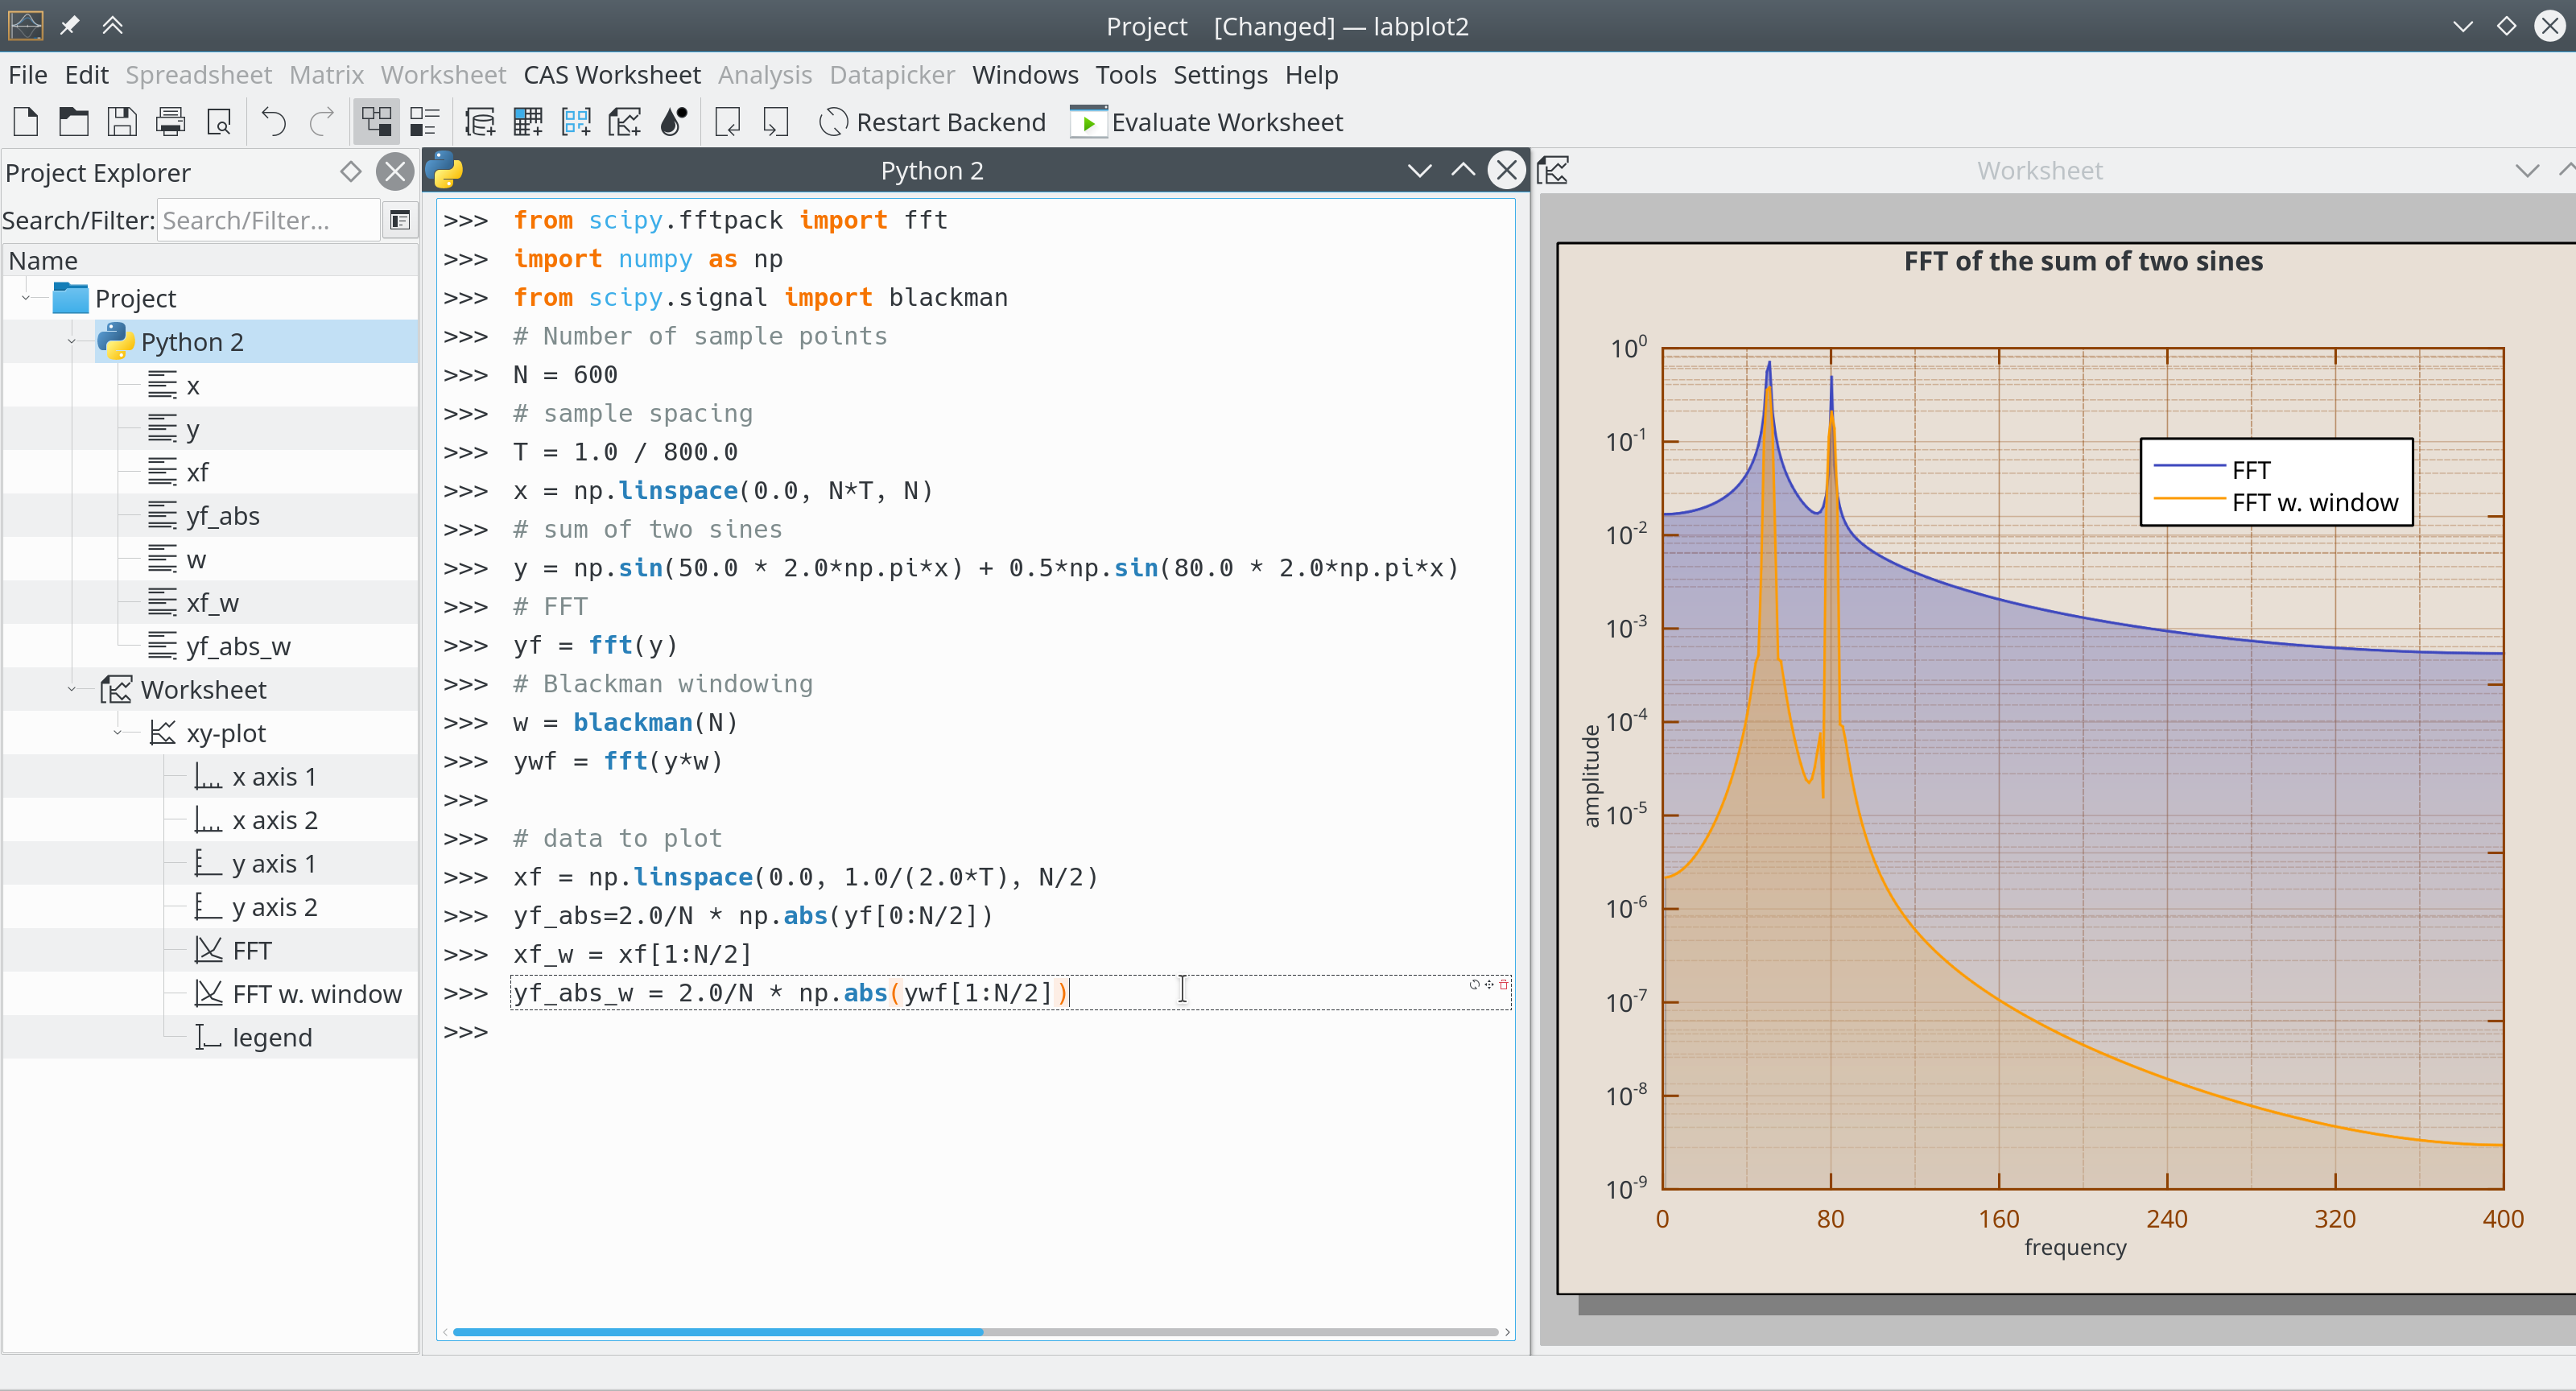
\includegraphics[width=\textwidth]{images/python_session.png}
\caption{Python session illustrating the effect of Blackman windowing on the Fourier transform}
\end{figure}



\chapter{Import and Export}
\section{Import}
\section{Export}

\chapter{Latex Typesetting}

\chapter{Tools}
\section{Curve Tracing}
\textit{Datapicker} is a tool that allows to easily extract data from image files. The process of extraction consists mainly out of the following steps:
\begin{itemize}
\item Import an image containing plots and curves where you want to read the data points from
\item Select the plot type (cartesian, polar, etc) 
\item Select tree reference points and provide values for them. With the help of these points the logical coordinate system is determined
\item Create a new datapicker curve and set the type of the error bars.
\item Switch to the mouse mode "Set Curve Points" and start selecting points on the imported image - the coordinates for the selected points are determined and added to the spreadsheet "Data".
\end{itemize}

It is possible to add more then one datapicker curve. This is useful in case the imported image contains several curves that need to be digitized.
The datapicker curve that is currently being selected in the Project Explorer is the "active" one - points clicked on the datapicker image will be calculated and added to its data spreadsheet.
\begin{figure}
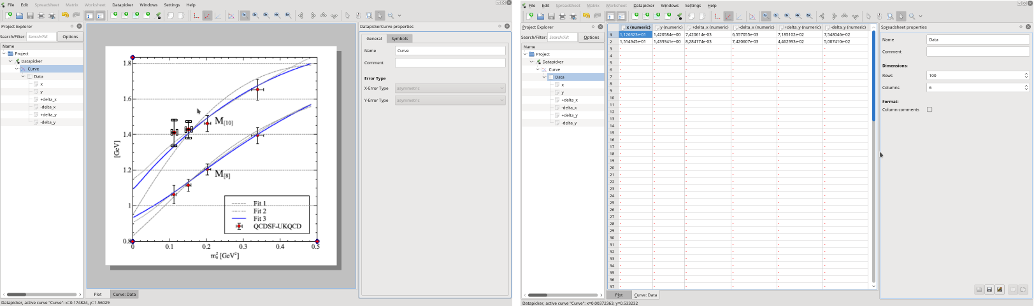
\includegraphics[width=\textwidth]{images/datapicker_active_curve_data_spreadsheet.png}
\caption{Coordinates of the digitized data points stored in a spreadsheet}
\end{figure}

Calculated values are stored in different columns in data spreadsheets in the datapicker. These columns behave exactly the same like other columns
in usual spreadsheets and can be directly used as source columns for curves in the plots.

Datapicker supports the process of the data extraction with several helpers. To place the points more precisely, a magnification glass with different magnification levels is available.
Also, the last selected point can be shifted with the help of the navigation keys.
Furthermore, when reading data points having error bars, datapicker automatically creates bars indicating the end points of the error bars.
Those bars can be pulled with the mouse until the required length (the distance to the data point) is reached.

The procedure for the extraction of data from an imported plot as described above is feasible when dealing with a limited number of points.
In case the curves in the imported image are given as solid lines, the datapicker tool in LabPlot allows to read them semi-automatically.
For this, after a new datapicker curve was added as described above, switch to the mouse mode "Select Curve Segments". The curves on the plot are recognized and highlighted.
By clicking on a highlighted curve (or one of its segments), points along this curve are created.
The length of a segment and the density of created points (separation between two points) are adjustable parameters.
On the screenshots below, after switching to the segment mode all black lines were highlighted (green colour).
In this specific case, the curve was recognized as a single segment and a single mouse-click on this segment is sufficient to digitize this curve and to automatically place points along the curve.
\begin{figure}
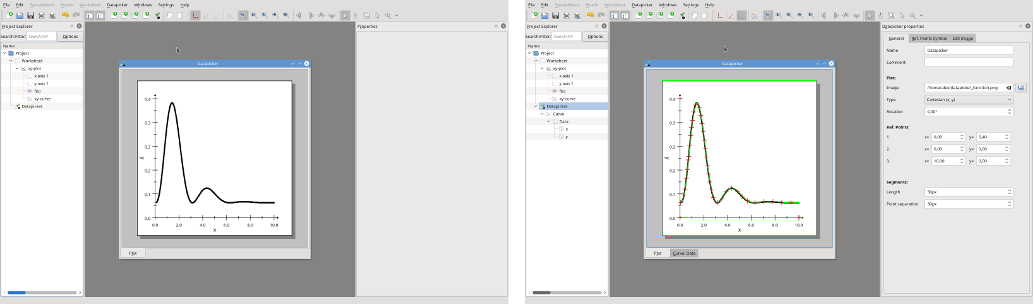
\includegraphics[width=\textwidth]{images/datapicker_segments.png}
\caption{Automatic creation of points along the recognized curve.}
\end{figure}

In many cases the plot is not as simple as above (single black curve on white background) and contains grid lines, many curves of different colour and thinness and a non-white background.
In such a case the automatic detection fails (too many or no objects are highlighted). To help the datapicker to determine the curve(s) correctly, the user has to limit the allowed ranges in the HSV (or HSI) colour spaces.
To subtract the non-white background it is possible to limit the range for the foreground colour, too.
Internally, each pixel of the image is converted to black and white where only the points fitting into the user-defined ranges for hue, saturation, value, intensity and foreground are set to black.

On the screenshots below, the blue curves in the original image were projected onto by having appropriately reduced the allowed ranges in the colour space (note the peak for blue in the histogram for the hue).
The transformed black and white image contains only the curves the user is interested in and it is now an easy task for the datapicker to determine the curves and to place points on them.
\begin{figure}
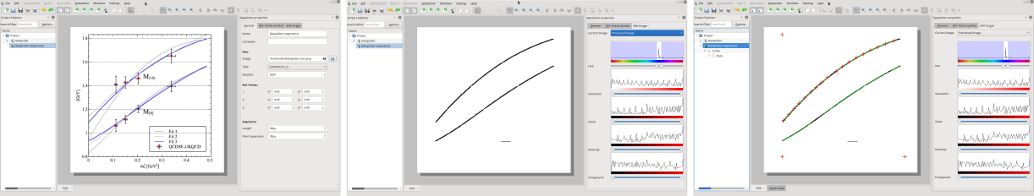
\includegraphics[width=\textwidth]{images/datapicker_original_transformed_segments.png}
\caption{Original image, image with the reduced color space and automatically created points for the recognized curve.}
\end{figure}

Similar to Worksheet, the currently visible area in the datapicker can be exported. The supported image formats as described in the section "Export".


\section{FITS Metadata Editor}
